\documentclass{article}

\usepackage{mathtools,amsfonts}
\usepackage{enumerate}
\usepackage{fullpage}
\usepackage{fancyvrb}
\usepackage{hyperref}


\begin{document}
\thispagestyle{empty}

\begin{center}
  \textbf{\Large Intermediate February Monthly Assignment}
  \\ \vspace{1em}
  \textbf{\large Due date: 20 February 2021}
\end{center}

\vspace{12pt}

\begin{enumerate}[1.]

\vspace{6pt}
\item % Jon
The natural number $n$ can be replaced by $ab$ if $a + b = n$, where $a$ and $b$ are natural numbers. Can the number $2021$ be obtained from $22$ after a sequence of such
replacements?


\vspace{6pt}
\item % Danielle/Taariq
Let $c$ and $d$ be positive divisors of a natural number $n$ such that $c > d$. Prove that $$c > d + \frac{d^2}{n}.$$


\vspace{6pt}
\item % Salvador 2017 9th grade Q2
Let $a$ and $b$ be positive real numbers such that $2a^2 +2b^2 = 5ab$.
If $|x|$ denotes the absolute value of $x$, calculate
\[ \left|\frac{a+b}{a-b}\right|. \]


\vspace{6pt}
\item % Taariq, stolen from AOPS
Triangle $ABC$ is a right angled triangle with $\angle C = 90^{\circ}$. $P$ is placed randomly inside $\triangle ABC$. What is the probability that the area of $\triangle PBC$ is less than half of the area of $\triangle ABC$?
\begin{figure}[h]
\centering
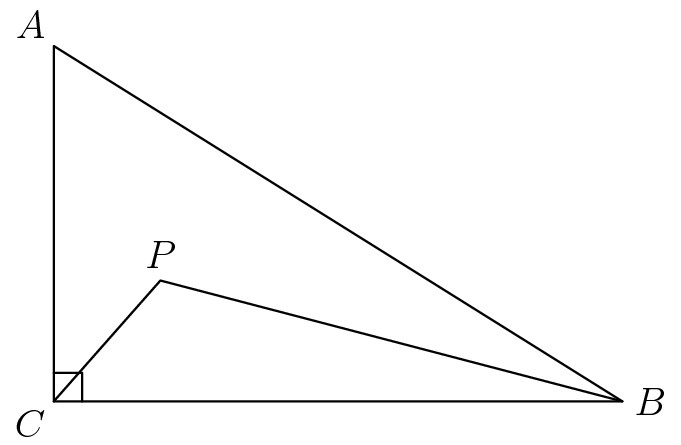
\includegraphics[width=0.5\textwidth]{fig.jpg}
\end{figure}


\vspace{6pt}
\item % DB-2014-1
Prove that among the first $30000$ positive integers there are at least $22000$ composite numbers.


\vspace{6pt}
\item % Ireland 2018 Q9
Suppose $a,b,c > 0$ and $\sqrt{a-b} +\sqrt{a-c} > \sqrt{b+c}$. Prove that $a > \dfrac{3}{4} (b+c)$.


\end{enumerate}


\vfill
\begin{itemize}
	\item Submit your solutions at \url{https://forms.gle/Kx1QDxDT5xP3Ez547}.
	\item Submit each question in a single separate PDF file (with multiple pages if necessary).
	\item If you take photographs of your work, use a document scanner such as Office Lens to convert to PDF.
	\item If you have multiple PDF files for a question, combine them using software such as PDFsam.
\end{itemize}

\end{document}
